\appendix

\section{Proofs}
\label{app:proofs}
Throughout the proofs, a logical form $\ell$ is a conjunctive query: a set of triple patterns over entities and variables with one answer variable, optionally with filters on bound values. For a triple set $\mathcal{S}$, $\operatorname{SPARQL}(\ell,\mathcal{S})$ is the set of values of the answer variable over all assignments that map every pattern of $\ell$ to a triple in $\mathcal{S}$ and satisfy the filters. Such queries are monotone: $\mathcal{S}\subseteq\mathcal{S}'$ implies $\operatorname{SPARQL}(\ell,\mathcal{S})\subseteq\operatorname{SPARQL}(\ell,\mathcal{S}')$. Following Definition 2, $\mathcal{S}$ \emph{supports} $(\ell,y)$ if $y\in\operatorname{SPARQL}(\ell,\mathcal{S})$, and a trajectory $\tau$ is \emph{evidence-covered} if $\operatorname{Cov}(\tau,\mathcal{S}^{*}_{q})=1$, as defined in Equation~\ref{eq:cov}.

\subsection{Proof of Proposition 1}
\label{app:proof1}
\textbf{Proposition 1.} \textit{Backward expansion preserves the answer and yields triples that support it.}\vspace{-2mm}
\begin{proof}
We show by induction that, for every $n\ge 1$, the triple set $\mathcal{S}^{(n)}\subseteq\mathcal{T}$ supports $(\ell^{(n)},y)$.

\textit{Base case.} A seed is retained only if its supporting triples exist in the KG and instantiate $\ell^{(1)}$ with the answer variable bound to $y$. Hence $\mathcal{S}^{(1)}$ supports $(\ell^{(1)},y)$ under some assignment $\mu$.

\textit{Inductive step.} Assume that $\mathcal{S}^{(n)}$ supports $(\ell^{(n)},y)$ under an assignment $\mu$. An expansion selects an entity $u$ in $\ell^{(n)}$ and a verified sub-question with logical form $\tilde{\ell}$, answer variable $x$, and triples $\tilde{\mathcal{S}}\subseteq\mathcal{T}$ that support $(\tilde{\ell},u)$ under an assignment $\tilde{\mu}$ with $\tilde{\mu}(x)=u$. With variables renamed apart, the expanded logical form is
\begin{equation}
    \ell^{(n+1)} = \ell^{(n)}[u\mapsto x]\;\cup\;\tilde{\ell},
\end{equation}
where $[u\mapsto x]$ replaces every occurrence of $u$ with the variable $x$. Consider the assignment $\mu\cup\tilde{\mu}$. Every pattern of $\tilde{\ell}$ is mapped into $\tilde{\mathcal{S}}$, and every pattern of $\ell^{(n)}[u\mapsto x]$ is mapped to the same triple of $\mathcal{S}^{(n)}$ as under $\mu$, since $\tilde{\mu}(x)=u$. The answer variable is still bound to $y$, which gives
\begin{equation}
    y\in\operatorname{SPARQL}\bigl(\ell^{(n+1)},\,\mathcal{S}^{(n+1)}\bigr),
\end{equation}
where $\mathcal{S}^{(n+1)}=\mathcal{S}^{(n)}\cup\tilde{\mathcal{S}}$, so $\mathcal{S}^{(n+1)}$ supports $(\ell^{(n+1)},y)$. Since $\mathcal{S}^{(n+1)}\subseteq\mathcal{T}$, monotonicity also gives $y\in\operatorname{SPARQL}(\ell^{(n+1)},\mathcal{T})$, so the answer is preserved over the full KG. Each expansion replaces one entity with a variable, so $N$ expansions hide $N$ intermediate entities.

The proof guarantees that the accumulated triples are sufficient for the answer, not that they are the only triples that support it. In the special case where the sub-question has answers other than $u$, the result set of $\ell^{(n+1)}$ may grow, but the executability check bounds it by $K_{\text{ans}}$.

In conclusion, every expansion keeps $y$ in the result set over the full KG, and the accumulated triples alone support the expanded logical form. Therefore, backward expansion preserves the answer and yields triples that support it.
\end{proof}

\subsection{Proof of Proposition 2}
\label{app:proof2}
\textbf{Proposition 2.} \textit{ECPR is maximized only by supported answers and rewards each triple once.}\vspace{-2mm}
\begin{proof}
Let $R=R_{\text{out}}+R_{\text{step}}+R_{\text{ecpr}}$ be the composite reward with $\lambda_{\text{ecpr}}>0$, and let $\mathcal{S}^{*}_{q}$ be the supporting triples of a question $q$, which support $(\ell_q,y_q^{*})$ by Proposition 1.

\textit{Supported maximizers.} Since $\operatorname{F1}\le 1$, $R_{\text{step}}\le\lambda_{\text{step}}$, and $\operatorname{Cov}\le 1$, the composite reward is bounded as
\begin{equation}
    R(\tau)\le\lambda_{\text{f1}}+\lambda_{\text{ret}}+\lambda_{\text{step}}+\lambda_{\text{ecpr}},
\end{equation}
where equality holds if and only if every term attains its maximum, in particular only if $\operatorname{Cov}(\tau,\mathcal{S}^{*}_{q})=1$. Assume that an evidence-covered trajectory with a correct answer and only valid actions is feasible within the turn limit. The bound is then attained, so every trajectory $\tau$ that maximizes $R$ satisfies $\mathcal{S}^{*}_{q}\subseteq\mathcal{T}(\tau)$, and monotonicity gives
\begin{equation}
    y_q^{*}\in\operatorname{SPARQL}\bigl(\ell_q,\,\mathcal{T}(\tau)\bigr),
\end{equation}
which means that the answer of $\tau$ is supported.

For outcome rewards alone, $R_{\text{out}}$ in Equation~\ref{eq:rout} depends on $\tau$ only through the prediction $\hat{y}$ and the returned entities $\mathcal{E}(\tau)$. A shortcut trajectory $\tau_s$ that predicts and reaches $y_q^{*}$ with $\operatorname{Cov}(\tau_s,\mathcal{S}^{*}_{q})<1$ therefore attains the maximum $\lambda_{\text{f1}}+\lambda_{\text{ret}}$ of $R_{\text{out}}$. Under the composite reward, it loses at least $\lambda_{\text{ecpr}}\bigl(1-\operatorname{Cov}(\tau_s,\mathcal{S}^{*}_{q})\bigr)>0$ against the bound and is no longer optimal.

\textit{One reward per triple.} Let $U_t=\bigl(\bigcup_{i\le t}\mathcal{T}_i\bigr)\cap\mathcal{S}^{*}_{q}$ be the gold triples retrieved up to step $t$, with $U_0=\emptyset$. The step reward of ECPR is then
\begin{equation}
    r^{\text{ecpr}}_{t}=\lambda_{\text{ecpr}}\,\frac{|U_t|-|U_{t-1}|}{|\mathcal{S}^{*}_{q}|},
\end{equation}
where $U_{t-1}\subseteq U_t$, so $r^{\text{ecpr}}_{t}\ge 0$ and the sum over steps telescopes to $\lambda_{\text{ecpr}}|U_T|/|\mathcal{S}^{*}_{q}|=R_{\text{ecpr}}(\tau)$. If step $t$ returns only triples that were already retrieved, then $U_t=U_{t-1}$ and $r^{\text{ecpr}}_{t}=0$. In contrast, every-match attribution pays $\lambda_{\text{ecpr}}|\mathcal{T}_t\cap\mathcal{S}^{*}_{q}|/|\mathcal{S}^{*}_{q}|$ at each step. Repeating a query that returns $m\ge 1$ gold triples for $T$ steps thus earns $\lambda_{\text{ecpr}}\,Tm/|\mathcal{S}^{*}_{q}|$, which grows with $T$ while the coverage stays at $m/|\mathcal{S}^{*}_{q}|$.

The statement concerns the maximizers of the trajectory-level reward and does not guarantee that policy optimization reaches them. Covering $\mathcal{S}^{*}_{q}$ is sufficient but not necessary for a supported answer, since a question may admit other supporting sets. In the special case where no shortcut trajectory exists for the question, the maximizers of $R_{\text{out}}$ are already evidence-covered, so the two rewards share the same maximizers.

In conclusion, the composite reward attains its maximum only when the retrieved triples support the answer, and first-match attribution never pays a triple twice. Therefore, ECPR is maximized only by supported answers and rewards each triple once.
\end{proof}

\section{FoG Algorithm Detail}
\label{app:redcheck}
\textbf{Redundancy Check.}
To provide a clear overview of the non-redundancy check in Section~\ref{sec:synthesis}, we present its procedure in the form of pseudocode. As shown in Algorithm~\ref{alg:redcheck}, we first build a support graph from the supporting triples and extract the shortest path from each topic entity to the answer node. We then enumerate proper subsets of topic entities in increasing size and execute one SPARQL query per subset. If any subset yields an answer set no larger than that of the full query, the question admits a shortcut and is discarded.

\begin{algorithm}[t]
\small
\caption{Redundancy Check}
\label{alg:redcheck}
\KwIn{\(\mathcal{S}^{(n)}\): supporting triples; \(E_q\): topic entities; \(\mathcal{Y}^{(n)}\): full answer set.}
\KwOut{Redundancy flag \(\textsc{IsRedundant}\in\{\text{True},\text{False}\}\).}

Build an undirected graph \(G\) from \(\mathcal{S}^{(n)}\); label topic-entity nodes with their Wikidata IDs, the answer node with \texttt{?answer}, and intermediates with fresh variables.\par

\For{each \(e \in E_q\)}{
    Compute shortest path \(\mathcal{P}(e)\) in \(G\) from \(e\) to the answer node.\par
    Derive SPARQL triple pattern \(\phi(e)\) from triples along \(\mathcal{P}(e)\).\par
}

\For{\(k = 1\) \textbf{to} \(|E_q|-1\)}{
    \For{each \(Z\subseteq E_q\) with \(|Z|=k\)}{
        \(Q_Z \leftarrow \texttt{SELECT\;?answer\;WHERE\;}\{\bigcup_{e\in Z}\phi(e)\}\)\par
        Execute \(Q_Z\) on the KG \(\rightarrow\) answer set \(\mathcal{Y}^{(n)}_Z\).\par
        \If{\(|\mathcal{Y}^{(n)}_Z|\le|\mathcal{Y}^{(n)}|\)}{
            \Return{\(\textsc{True}\)}
        }
    }
}

\Return{\(\textsc{False}\)}
\end{algorithm}

\textit{Complexity Analysis.}
Given a question with $|E_q|$ topic entities and $|\mathcal{S}^{(n)}|$ supporting triples, extracting the shortest paths by BFS takes $\mathcal{O}(|E_q|\cdot|\mathcal{S}^{(n)}|)$ time. The subset enumeration issues at most $2^{|E_q|}-2$ SPARQL queries and stops at the first redundant subset. Using only the shortest path per topic entity is an approximation, which we audit on 200 candidate questions against an exhaustive enumeration of all path combinations under the same hop limit. The shortest-path check misses a shortcut in 1.5\% of the candidates, while issuing 5.1 rather than 48.6 SPARQL queries per question.

In summary, the redundancy check is dominated by SPARQL execution, and the shortest-path approximation reduces the number of queries by 9.5$\times$ while missing few shortcuts.

\section{Synthetic Data Construction}
\label{app:data}

\subsection{Topic Domains}
\label{app:data_stats}
\begin{figure}[t]
    \centering
    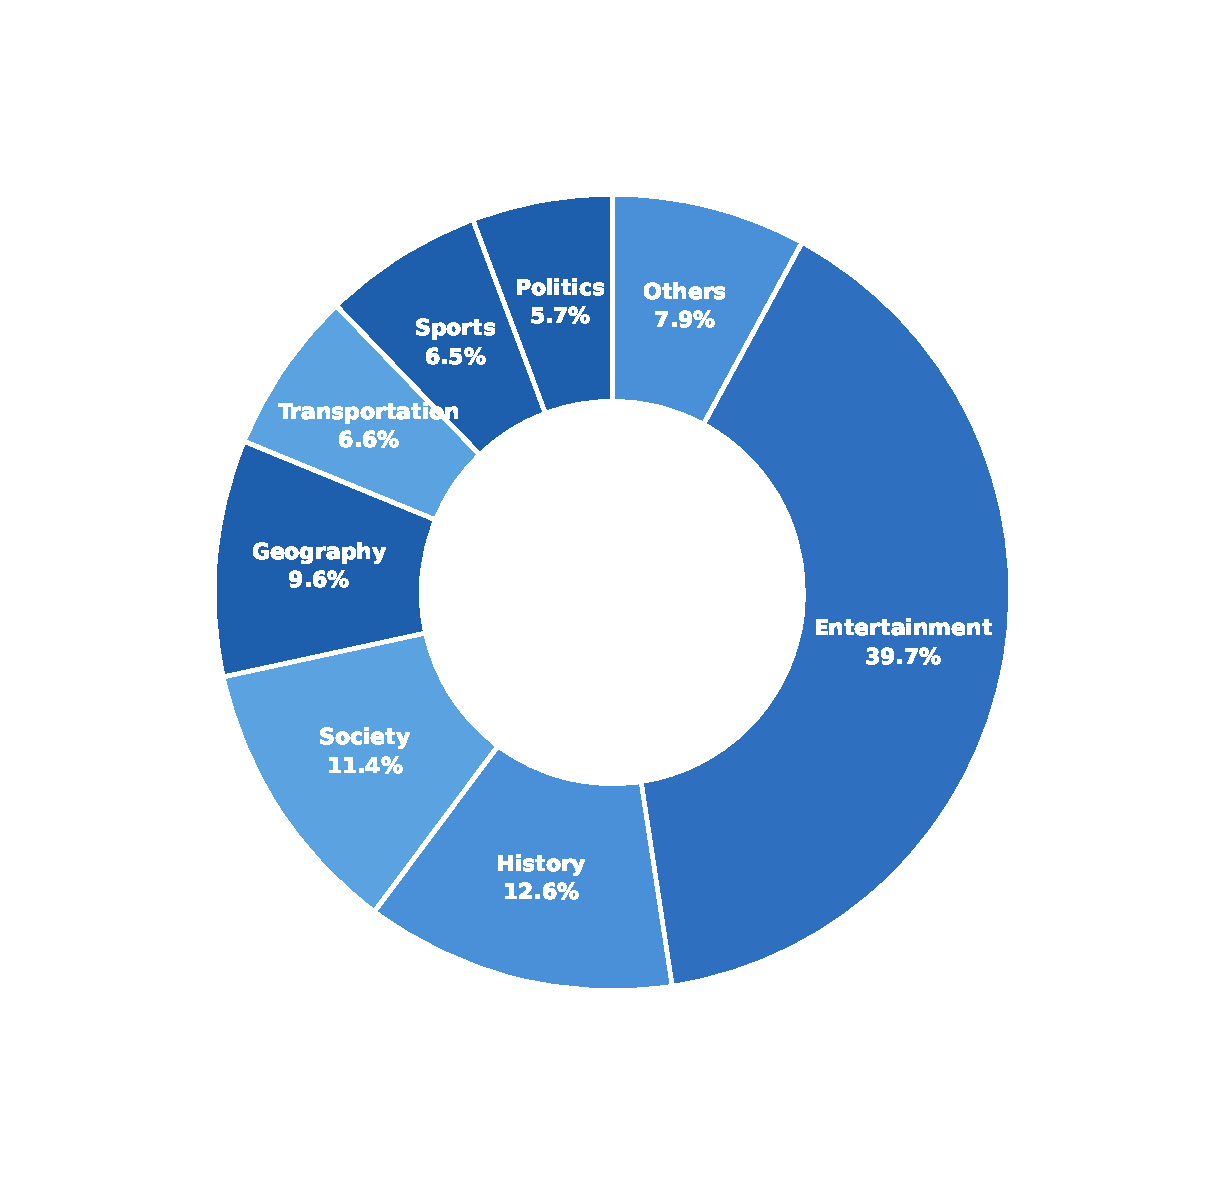
\includegraphics[width=1.0\linewidth]{figures/data_dist.pdf}
    \caption{\textbf{Topic-domain distribution of the synthetic questions.} The questions are drawn from major Wikidata domains.}
    \label{fig:data_dist}
\end{figure}
As shown in Figure~\ref{fig:data_dist}, the synthetic questions used for FoG training span seven named Wikidata domains. Entertainment is the largest (39.7\%), reflecting the density of film, television, and music entities in Wikidata, followed by history (12.6\%), society (11.4\%), geography (9.6\%), transportation (6.6\%), sports (6.5\%), and politics (5.7\%); the remaining 7.9\% fall into other domains.

\subsection{Query-Graph Topologies}
\label{app:iso_dist}
\begin{table}[t]
  \centering
  \small
  
  \begin{tabular}{clrr}
  \toprule
  \textbf{Hops} & \textbf{Isomorphism Type} & \textbf{Questions} & \textbf{Proportion} \\
  \midrule
  \multirow{3}{*}{1 hop}
    & \texttt{(1)}           & 500 & 7.59\% \\
    & \texttt{(1)(1)}        & 600 & 9.11\% \\
    & \texttt{(1)(1)(1)}     & 1,211 & 18.38\% \\
  \midrule
  \multirow{4}{*}{2 hop}
    & \texttt{(2)}           & 550 & 8.35\% \\
    & \texttt{(2)(1)}        & 853 & 12.95\% \\
    & \texttt{((1)(1))}      & 700 & 10.63\% \\
    & \texttt{(2)(1)(1)}     & 533 & 8.09\% \\
  \midrule
  \multirow{2}{*}{3 hop}
    & \texttt{(3)}           & 1,086 & 16.48\% \\
    & \texttt{((2)(1))}      & 555 & 8.42\% \\
  \midrule
  \textbf{Total} & - & \textbf{6,588} & \textbf{100.00\%} \\
  \bottomrule
  \end{tabular}
\caption{\textbf{Topology distribution of the synthetic questions.} Query-graph isomorphism types are grouped by hop count, the longest path from a topic entity to the answer.}
\label{tab:distribution}
  \end{table}

To construct questions with diverse reasoning structures, we label each synthetic question with the isomorphism type of its query graph. As shown in Table~\ref{tab:distribution}, the 6,588 questions that pass all checks span nine chain and tree structures from 1 to 3 hops. All verified seeds enter backward expansion, and the 1-hop questions are seeds retained at depth one. Overall, 35.1\%, 40.0\%, and 24.9\% of the questions have 1, 2, and 3 hops. The most frequent types are the three-branch star \texttt{(1)(1)(1)} (18.38\%) and the 3-hop chain \texttt{(3)} (16.48\%), and 67.6\% of the questions have a multi-branch query graph rather than a single chain.

\subsection{Synthesis Cost and Retention}
\label{app:synth_cost}
\begin{table}[t]
\centering
\small
\resizebox{\columnwidth}{!}{
\begin{tabular}{lrrrr}
\toprule
\textbf{Stage} & \textbf{Input} & \textbf{Retained} & \textbf{Rejected} & \textbf{Teacher calls} \\
\midrule
Seed-question generation        & 20,000 & 14,400 & 28.0\% & 20,000 \\
Backward expansion              & 14,400 & 8,784  & 39.0\% & 86,400 \\
Complex-question composition    & 8,784  & 6,588  & 25.0\% & 8,784 \\
\midrule
\textbf{End-to-end}             & 20,000 & 6,588  & 67.1\% & 115,184 \\
\bottomrule
\end{tabular}}
\caption{\textbf{Synthesis cost and retention.}}
\label{tab:synth_cost}
\end{table}

As shown in Table~\ref{tab:synth_cost}, we report the candidates retained, the rejection rate, and the teacher calls at each synthesis stage, all of which use the same teacher model, Kimi-K2~\citep{kimi}. Of 20,000 sampled seed entities, 14,400 yield a verified seed question, 8,784 candidates remain after backward expansion, and 6,588 questions pass all filters, an end-to-end rejection rate of 67.1\%. The pipeline uses 115,184 teacher calls, about 17.5 per retained question, and backward expansion accounts for three quarters of them.

\subsection{Data Leakage Check}
\label{app:leakage}
To ensure that the synthetic questions do not overlap with the test sets, we encode each question with BGE-M3 and compute the cosine similarity between every test question and its most similar synthetic question. The similarity stays below 0.85 for all test questions. On QALD10-en and WikiWebQuestions, no test question exceeds 0.75, and on GTSQA only 6 questions (0.37\%) fall in the 0.80--0.85 range.

\section{KG Interaction Operations}
\label{app:kg_ops}
\begin{table*}[t]
\centering
\small

\resizebox{\textwidth}{!}{         
\begin{tabular}{>{\centering\arraybackslash}m{2.5cm} m{3.8cm} m{5.0cm} m{3.5cm} m{2.2cm}}
\toprule
\textbf{Category} & \textbf{Function} & \textbf{Description} & \textbf{Input Parameters} & \textbf{Output} \\
\midrule
\multirow{2}{2.5cm}{\centering Relation search}
  & \texttt{find\_outgoing\_relations}
  & Given an entity, return all outgoing relations.
  & \texttt{entity\_name}
  & List of outgoing relations \\[4pt]
  & \texttt{find\_incoming\_relations}
  & Given an entity, return all incoming relations.
  & \texttt{entity\_name}
  & List of incoming relations \\
\midrule
\multirow{2}{2.5cm}{\centering Neighborhood expansion}
  & \texttt{get\_tail\_entities}
  & Follow the relation forward from head to tail.
  & \texttt{head\_entity\_name}; \texttt{relation\_name}
  & Set of tail entities \\[4pt]
  & \texttt{get\_head\_entities}
  & Follow the relation backward from tail to head.
  & \texttt{tail\_entity\_name}; \texttt{relation\_name}
  & Set of head entities \\
\midrule
\multicolumn{1}{>{\centering\arraybackslash}m{2.5cm}}{Constraint filtering}
  & \texttt{get\_entity\_by\_constraint}
  & Filter the provided \texttt{entity\_set} and return the entities satisfying the specified constraint.
  & \texttt{entity\_set}; \texttt{relation}; \texttt{operator}; \texttt{value}
  & Entity subset \\
\midrule
\multirow{2}{2.5cm}{\centering Set combination}
  & \texttt{intersect}
  & Return the intersection of the given list of entity sets.
  & \texttt{entity\_set\_list}
  & Intersection set \\[4pt]
  & \texttt{union}
  & Return the union of the given list of entity sets.
  & \texttt{entity\_set\_list}
  & Union set \\
\bottomrule
\end{tabular}}
\caption{\textbf{The seven KG operations of the \texttt{kg-query} action.} Each operation is listed with its description, input parameters, and output.}
\label{tab:kg_operations}

\end{table*}


As shown in Table~\ref{tab:kg_operations}, the \texttt{kg-query} action in Section~\ref{sec:agent} is instantiated with seven operations in four categories: relation search, neighborhood expansion, constraint filtering, and set combination. The table lists the name, description, input parameters, and output of every operation.

\section{Benchmark Datasets}
\label{app:datasets}
\label{app:datasets_detail}
The benchmarks used for FoG evaluation cover two knowledge graphs, with data sourced as follows:

\textbf{WikiWebQuestions:} Ported from WebQuestions and re-annotated with SPARQL queries over Wikidata~\cite{wikiwebQuestions}, consisting of real-world natural language questions.

\textbf{QALD10-en:} Derived from the English subset of the tenth QALD challenge~\cite{qald10en}, the first edition to adopt Wikidata, covering 394 expert-written test questions with multi-hop and qualifier constraints.

\textbf{GTSQA:} Built over Wikidata with 30,144 training and 1,622 test questions~\cite{GTSQA}, each annotated with a gold answer subgraph and a query-graph isomorphism label.

\textbf{WebQSP:} Sourced from Freebase~\cite{webqsp} and used only for the zero-shot cross-KG transfer experiment.

\section{Evaluation Details}
\label{app:evaluation}

\subsection{Evaluation Metrics}
\label{app:metrics}
We evaluate model performance using four complementary metrics that assess two aspects of KGQA: answer accuracy (Hit@1 and F1) and evidence coverage (Cov and RetQ).

\textbf{(i) Hit@1.}
Hit@1 quantifies whether the predicted answer is correct. For each question, we check whether the normalized prediction matches any gold answer, and then average over all evaluated questions:
\begin{equation}
\begin{aligned}
    \mathrm{Hit@1} = \frac{1}{M}\sum_{i=1}^{M}
        \mathbb{I}\bigl[&\exists y \in Y_i^{*}: \\
        &\mathrm{norm}(\hat{y}_i) = \mathrm{norm}(y)\bigr],
\end{aligned}
\end{equation}
where $\hat{y}_i$ and $Y_i^{*}$ denote the prediction and the gold answer set of the $i$-th question, $\mathrm{norm}(\cdot)$ removes superficial differences such as case and punctuation, and $M$ is the total number of evaluated questions in the benchmark.

\textbf{(ii) Token-level F1.}
F1 quantifies the token-level overlap between the predicted and gold answers. For each question, we compute the harmonic mean of token precision and recall, and then average:
\begin{equation}
\small
    \mathrm{F1} = \frac{1}{M}\sum_{i=1}^{M}
        \dfrac{2\cdot\left|\mathrm{tokens}(\hat{y}_i) \cap \mathrm{tokens}(Y_i^{*})\right|}
             {\left|\mathrm{tokens}(\hat{y}_i)\right| + \left|\mathrm{tokens}(Y_i^{*})\right|},
\end{equation}
where $\mathrm{tokens}(\cdot)$ normalizes each answer in a list, splits it on whitespace, and takes the union of the resulting tokens over the list.

\textbf{(iii) Evidence Coverage (Cov).}
Cov quantifies how much of the gold supporting evidence the agent retrieves along its trajectory. For each question, we compute the fraction of gold supporting triples returned by its KG queries, and then average over all questions:
\begin{equation}
    \mathrm{Cov} = \frac{1}{M}\sum_{i=1}^{M}
        \frac{|\mathcal{T}(\tau_i) \cap \mathcal{S}^{*}_{i}|}
             {|\mathcal{S}^{*}_{i}|},
\end{equation}
where $\mathcal{T}(\tau_i)$ denotes the set of triples returned by all \texttt{kg-query} actions in the trajectory $\tau_i$, and $\mathcal{S}^{*}_{i}$ denotes the gold supporting triples of the $i$-th question. This metric reflects whether an answer is backed by the complete evidence path.

\textbf{(iv) Retrieval Grounding (RetQ).}
RetQ quantifies whether the gold answer is retrieved from the KG rather than produced from parametric memory. For each question, we check whether any gold answer appears among the entities returned by its KG queries, and then average over all questions:
\begin{equation}
    \mathrm{RetQ} = \frac{1}{M}\sum_{i=1}^{M}
        \mathbb{I}\!\left[\exists y \in Y_i^{*},\; y \in \mathcal{E}(\tau_i)\right],
\end{equation}
where $\mathcal{E}(\tau_i)$ denotes the set of entities returned by all KG queries in the trajectory $\tau_i$.

\subsection{Gold Supporting Triples}
\label{app:gold_supporting_triples}
The gold supporting triples used for evaluation are distinct from those produced by synthesis, which serve only as ECPR supervision during training. GTSQA provides gold answer subgraphs natively. For WikiWebQuestions, which has no such annotation, we follow EoG~\cite{EoG} and construct them in two stages. We first enumerate candidate paths from each topic entity to each answer entity by BFS under a maximum-hop constraint. An LLM verifier then judges whether each candidate path supports all constraints of the question, and the union of triples on the accepted paths forms the gold supporting triples.

\subsection{Human Validation of Constructed Paths}
\label{app:human_audit}
\begin{table*}[t]
\centering
\small
\begin{tabular}{p{4.2cm} p{5.6cm} p{5.2cm}}
\toprule
\textbf{Question} & \textbf{Candidate path} & \textbf{Reason for rejection} \\
\midrule
Who was the prime minister of Pakistan in 1999?
& Links candidates only to the office ``Prime Minister of Pakistan''.
& Does not establish that the candidate held the office in 1999. \\
\midrule
What town did Justin Bieber grow up in?
& Justin Bieber $\rightarrow$ Canada; Waterloo $\rightarrow$ Canada.
& Sharing the same country does not establish childhood residence. \\
\bottomrule
\end{tabular}
\caption{\textbf{Representative rejected paths.} The verifier checks whether a path covers the semantic constraints of the question, not only whether it reaches a plausible answer entity.}
\label{tab:rejected_paths}
\end{table*}

To validate the constructed paths independently of the LLM verifier, we sample 200 candidate paths from WikiWebQuestions, 100 accepted and 100 rejected by the verifier. Three graduate annotators independently judge whether each path supports all constraints of its question, without seeing the verifier decision. The annotators reach Fleiss' $\kappa=0.91$, and the human--verifier agreement is 93.0\%, with a verifier precision of 0.94 and a recall of 0.92. Table~\ref{tab:rejected_paths} shows two representative rejected paths.

\section{Baseline Details}
\label{app:baselines}
We compare FoG against nine representative baselines that cover the LLM reasoning, retrieval-based, and agent-based paradigms:

\textbf{IO Prompt}~\cite{gpt-4,qwen,deepseekv3} is a KG-free baseline where the LLM directly answers the question from its parametric knowledge. This serves as a lower bound for KG-augmented reasoning.

\textbf{CoT}~\cite{CoT} elicits step-by-step reasoning before the final answer, still without any access to the KG.

\textbf{Self-Consistency}~\cite{Self-Consistency} samples multiple CoT chains and aggregates their answers by majority voting.

\textbf{RoG}~\cite{RoG} generates relation paths as plans, retrieves reasoning paths along them, and answers from the retrieved paths.

\textbf{SubGraphRAG}~\cite{SubGraphRAG} retrieves a subgraph with a lightweight MLP that scores triples in parallel, and feeds it to an LLM reader.

\textbf{GCR}~\cite{GCR} encodes KG paths into a Trie index and constrains LLM decoding with the graph structure.

\textbf{ToG}~\cite{ToG} is a training-free agent that performs beam search over entities and relations through multi-turn KG interaction.

\textbf{PoG}~\cite{PoG} decomposes the question into sub-objectives and explores paths with memory updating and self-reflection.

\textbf{KG-R1}~\cite{KG-R1} trains a single KG agent end-to-end with GRPO under outcome and turn-level action-validity rewards.

\textbf{Adaptation to Wikidata.}
RoG, SubGraphRAG, and GCR were proposed on Freebase and rely on dataset-specific supervision, so they cannot be transferred to a new KG without retraining. We therefore retrain each of them on the training split of every Wikidata benchmark. KG-R1 was also proposed on Freebase. We retrain it on Wikidata with the same training data as FoG.

\label{app:inference_setting}
To ensure fairness, all methods, including FoG, are evaluated under identical conditions with a single inference run per question, and no multi-run aggregation is used. The backbone of each method is listed in Table~\ref{tab:main_result}.

\section{Hyperparameter Settings}
\label{app:training}
\textbf{Supervised Fine-Tuning.}
\label{app:sft}
For SFT, we adopt LLaMA-Factory~\cite{zheng2024llamafactory} and apply LoRA to all linear layers. The training trajectories are distilled from the same teacher model used in synthesis, Kimi-K2~\cite{kimi}, with the prompt in Table~\ref{tab:traj_gen_prompt}. Training runs on a single NVIDIA A100 GPU.

\begin{table}[t]
\centering
\small

\resizebox{\columnwidth}{!}{         
\begin{tabular}{lc}
\toprule
\textbf{Parameter} & \textbf{Value} \\
\midrule
Fine-tuning method       & LoRA \\
LoRA rank / alpha / dropout & 16 / 32 / 0.05 \\
Max sequence length      & 3,000 \\
Training epochs          & 3 \\
Per-device batch size    & 16 \\
Gradient accumulation steps & 8  \\
Learning rate            & $5\times10^{-5}$ \\
LR scheduler             & Cosine, warmup ratio 0.1 \\
Weight decay             & 0.01 \\
Gradient clipping        & 1.0 \\
\bottomrule
\end{tabular}}
\caption{\textbf{Hyperparameters of supervised fine-tuning.}}
\label{tab:sft_hyperparams}
\end{table}


\textbf{Reinforcement Learning.}
\label{app:rl}
For RL, we adopt Verl~\cite{sheng2025hybridflow} and initialize the policy from the SFT checkpoint. Training runs on a single node with 4$\times$NVIDIA A100 (40\,GB) GPUs, using FSDP with parameter and optimizer CPU offloading, and rollouts are executed with vLLM. For each question, the agent samples $N{=}4$ trajectories with at most 10 KG interaction turns. KL regularization uses the $k_3$ estimator with coefficient 0.03, anchored to the SFT model. Table~\ref{tab:sft_hyperparams} and Table~\ref{tab:rl_hyperparams} summarize the detailed hyperparameter configurations used throughout our experiments, and Table~\ref{tab:reward_weights} lists the coefficients of the composite reward in Section~\ref{sec:training}.

\textbf{Advantage Computation.}
\label{app:advantage}
The turn-level advantage in Section~\ref{sec:training} is computed as follows.
\textit{(i) Return.} The return $G_{i,t}$ in Equation~\ref{eq:turn_return} adds the immediate process rewards of turn $t$ to the outcome reward of the trajectory. We use neither discounting nor a reward-to-go, so the evidence reward of a turn is credited to that turn only.
\textit{(ii) Normalization.} The mean $\mu_q$ and standard deviation $\sigma_q$ are computed over all (trajectory, turn) pairs of the $N$ rollouts of the same question. Trajectories of different lengths need no padding, since each contributes as many returns as it has turns.
\textit{(iii) Token mask.} The advantage of a turn is broadcast to the tokens that the policy generates in that turn, i.e., its reasoning and its tool call or answer. Tool observations are part of the context but are masked out of the policy loss and the KL term.
\textit{(iv) Objective.} The policy maximizes
\begin{equation}
\small
\begin{aligned}
&\mathcal{J}(\theta)
= \mathbb{E}_{q,\{\tau_i\}}
\Bigg[
\frac{1}{N}\sum_{i=1}^{N}\frac{1}{|\tau_i|}\sum_{j=1}^{|\tau_i|}
\min \Big(
\rho_{i,j}\hat{A}_{i,t(j)}, \\
&\quad\operatorname{clip}(\rho_{i,j}, 1-\epsilon, 1+\epsilon)\hat{A}_{i,t(j)}
\Big)
\Bigg]
- \beta \,\mathbb{D}_{\mathrm{KL}}(\pi_{\theta}\,\|\,\pi_{\text{ref}}),
\end{aligned}
\end{equation}
where $j$ ranges over the $|\tau_i|$ policy-generated tokens, $t(j)$ is the turn of token $j$, $\rho_{i,j}$ is the probability ratio, and $\pi_{\text{ref}}$ is the SFT model.
\textit{(v) Difference from trajectory-level credit.} When the coverage reward is credited only to the final turn, the turns that actually retrieved the evidence receive the same return as the turns that did not, so the update cannot distinguish them. With first-match attribution, two trajectories with the same coverage still produce different per-turn returns, and the advantage concentrates on the queries that first reach gold triples.

\begin{table}[t]
\centering
\small

\resizebox{\columnwidth}{!}{         
\begin{tabular}{lc}
\toprule
\textbf{Parameter} & \textbf{Value} \\
\midrule
Actor learning rate           & $1\times10^{-6}$ \\
KL loss coefficient           & 0.03 ($k_3$ type) \\
GRPO rollout $N$              & 4 \\
Max interaction turns per question & 10 \\
Train batch size              & 32 \\
PPO mini-batch size           & 16 \\
Max prompt length             & 4,096 \\
Max response length per step  & 8,192 \\
Max observation length        & 1,024 \\
Rollout temperature           & 0.7 \\
Total training steps          & 450 \\
Hardware                      & 4$\times$ NVIDIA A100 (40\,GB) \\
\bottomrule
\end{tabular}}
\caption{\textbf{Hyperparameters of reinforcement learning.}}
\label{tab:rl_hyperparams}
\end{table}

\begin{table}[t]
\centering
\small
\begin{tabular}{llc}
\toprule
\textbf{Reward term} & \textbf{Coefficient} & \textbf{Value} \\
\midrule
Answer F1 ($R_{\text{out}}$)          & $\lambda_{\text{f1}}$   & 0.7 \\
Answer retrieval ($R_{\text{out}}$)   & $\lambda_{\text{ret}}$  & 0.3 \\
Step validity ($R_{\text{step}}$)     & $\lambda_{\text{step}}$ & 0.5 \\
Evidence coverage ($R_{\text{ecpr}}$) & $\lambda_{\text{ecpr}}$ & 1.0 \\
\bottomrule
\end{tabular}
\caption{\textbf{Coefficients of the composite reward.} Each coefficient weights one term of the reward in Section~\ref{sec:training}.}
\label{tab:reward_weights}
\end{table}


\section{Case Study}
\label{app:casestudy}
To better understand how much of the supporting evidence different methods retrieve from the KG, we present a case study on the question: \textit{``Which airline flies the Embraer 195 and is based at the airport named after Margaret Kenyatta's father?''} As shown in Tables~\ref{tab:fogcase}, \ref{tab:togcase}, and~\ref{tab:pogcase}, this question requires resolving the father, the airport named after him, and the airline that is based there and flies the aircraft. All three methods predict the correct answer, but they differ in how much of the evidence chain they recover.

\textbf{FoG} recovers the complete gold evidence. It issues nine KG turns and grounds each hop in the triples returned by the previous one, so every link of the chain can be read from the trajectory.

In contrast, \textbf{ToG} performs four rounds of beam search but recovers only one relevant triple, missing the links for airport naming and airline hub, so its answer relies mainly on parametric knowledge. \textbf{PoG} answers after a single retrieval step, leaving an evidence chain that cannot be audited from the trajectory. This case highlights the strength of FoG in reaching the answer through evidence that is fully retrieved from the KG.

\begin{table*}[ht]
\centering
\footnotesize
\setlength{\tabcolsep}{8pt}
\renewcommand{\arraystretch}{1.3}
\caption{\textbf{Case study of FoG.} The trajectory recovers the complete gold evidence before answering.}

\begin{tabular}{>{\raggedright\arraybackslash}p{0.95\textwidth}}
\rowcolor{gray!20}
\textbf{Question:} Which airline flies the \textbf{Embraer 195} and is based at the airport named after \textbf{Margaret Kenyatta}'s father? \\[2pt]

\rowcolor{blue!10}
\texttt{<think>}I need to find an airline that satisfies two conditions: 1) flies the Embraer 195, and 2) is based at the airport named after Margaret Kenyatta's father. Let me start by exploring the relationships around the first given entity to understand what information is stored about Margaret Kenyatta in the knowledge graph.{</think>} \\

\rowcolor{green!10}
\texttt{<kg-query>} find\_outgoing\_relations(entity\_name=Margaret Kenyatta)  \texttt{</kg-query>} \\
\rowcolor{yellow!10}
\texttt{<information>} Outgoing relations for entity Margaret Kenyatta: country of citizenship, father, given name, instance of, mother, occupation, sex or gender......... \texttt{</information>} \\

\rowcolor{blue!10}
\texttt{<think>} The outgoing triple shows that Margaret Kenyatta has a "father" in the knowledge graph. Let me find out who her father is by querying the triple that directly connects Margaret Kenyatta to her father. {</think>} \\

\rowcolor{green!10}
\texttt{<kg-query>} get\_tail\_entities(head\_entity\_name=Margaret Kenyatta, relation\_name=father)  \texttt{</kg-query>} \\
\rowcolor{yellow!10}
\texttt{<information>} Entities outgoing via relation father from entity Margaret Kenyatta: Jomo Kenyatta.......... \texttt{</information>} \\

\rowcolor{blue!10}
\texttt{<think>} Now I know Jomo Kenyatta is Margaret Kenyatta's father. Next, I need to find the airport named after Jomo Kenyatta. Let me check what relationships exist for Jomo Kenyatta in the knowledge graph to see if there is an airport named after him. {</think>} \\

\rowcolor{green!10}
\texttt{<kg-query>} find\_incoming\_relations(entity\_name=Jomo Kenyatta) \texttt{</kg-query>} \\
\rowcolor{yellow!10}
\texttt{<information>} Incoming relations for entity Jomo Kenyatta: father,named after,spouse.......... \texttt{</information>} \\

\rowcolor{blue!10}
\texttt{<think>} I see that some entities have "named after" pointing to Jomo Kenyatta. Let me find out what entities are named after Jomo Kenyatta in the knowledge graph. {</think>} \\

\rowcolor{green!10}
\texttt{<kg-query>} get\_head\_entities(tail\_entity\_name=Jomo Kenyatta, relation\_name=named after)  \texttt{</kg-query>} \\
\rowcolor{yellow!10}
\texttt{<information>} Entities incoming via relation named after from entity Jomo Kenyatta: Jomo Kenyatta International Airport, Kenyatta International Convention Centre \texttt{</information>} \\

\rowcolor{blue!10}
\texttt{<think>}  Great! I found that Jomo Kenyatta International Airport is named after Jomo Kenyatta. Now I need to find which airline is based at Jomo Kenyatta International Airport. Let me check what outgoing relationships exist for Jomo Kenyatta International Airport to see if there is an airline based there. {</think>} \\

\rowcolor{green!10}
\texttt{<kg-query>} find\_outgoing\_relations(entity\_name=Jomo Kenyatta International Airport)  \texttt{</kg-query>} \\
\rowcolor{yellow!10}
\texttt{<information>} Outgoing relations for entity Jomo Kenyatta International Airport: country, instance of, located in the administrative territorial entity, named after......... \texttt{</information>} \\

\rowcolor{blue!10}
\texttt{<think>} I don't see a direct "airline based at" relationship listed for the airport. Let me check the incoming relationships to see if any airlines have "headquarters location" or similar relationships pointing to this airport. {</think>} \\

\rowcolor{green!10}
\texttt{<kg-query>} find\_incoming\_relations(entity\_name=Jomo Kenyatta International Airport).  \texttt{</kg-query>} \\
\rowcolor{yellow!10}
\texttt{<information>} Incoming relations for entity Jomo Kenyatta International Airport: airline hub \texttt{</information>} \\

\rowcolor{blue!10}
\texttt{<think>} Perfect! I found that some airlines have "airline hub" pointing to Jomo Kenyatta International Airport. Let me find out which airlines have Jomo Kenyatta International Airport as their airline hub. {</think>} \\

\rowcolor{green!10}
\texttt{<kg-query>} get\_head\_entities(tail\_entity\_name=Jomo Kenyatta International Airport, relation\_name=airline hub)  \texttt{</kg-query>} \\
\rowcolor{yellow!10}
\texttt{<information>} Entities incoming via relation airline hub from entity Jomo Kenyatta International Airport: Kenya Airways \texttt{</information>} \\

\rowcolor{blue!10}
\texttt{<think>} Now I have Kenya Airways as the airline based at Jomo Kenyatta International Airport. Finally, I need to verify that Kenya Airways also flies the Embraer 195. Let me check what aircraft types Kenya Airways operates by looking at its outgoing relationships. {</think>} \\

\rowcolor{green!10}
\texttt{<kg-query>} find\_outgoing\_relations(entity\_name=Kenya Airways)  \texttt{</kg-query>} \\
\rowcolor{yellow!10}
\texttt{<information>} Outgoing relations for entity Kenya Airways: airline alliance, airline hub, country, instance of, item operated .........\texttt{</information>} \\

\rowcolor{blue!10}
\texttt{<think>} I see that Kenya Airways has "item operated" as an outgoing relationship. Let me find out what items (likely aircraft) Kenya Airways operates. {</think>} \\

\rowcolor{green!10}
\texttt{<kg-query>} get\_tail\_entities(head\_entity\_name=Kenya Airways, relation\_name=item operated)  \texttt{</kg-query>} \\
\rowcolor{yellow!10}
\texttt{<information>} Entities outgoing via relation item operated from entity Kenya Airways: Boeing 737 Classic,Boeing 737 Next Generation,Boeing 767,Boeing 777,Boeing 787 Dreamliner,Embraer 195 \texttt{</information>} \\

\rowcolor{blue!10}
\texttt{<think>}  I now have enough grounded evidence to give the answer. \texttt{</think>} \\

\rowcolor{green!30}
\texttt{<answer>} ["Kenya Airways"] \texttt{</answer>} \\
\end{tabular}

\label{tab:fogcase}
\end{table*}
\begin{table*}[ht]
\centering
\footnotesize
\setlength{\tabcolsep}{8pt}
\renewcommand{\arraystretch}{1.3}
\caption{\textbf{Case study of ToG.} The trajectory reaches the correct answer while covering only the first part of the gold evidence.}

\begin{tabular}{>{\raggedright\arraybackslash}p{0.95\textwidth}}
\rowcolor{gray!20}
\textbf{Question:} Which airline flies the \textbf{Embraer 195} and is based at the airport named after \textbf{Margaret Kenyatta}'s father? \\[4pt]

\rowcolor{blue!10}
\texttt{Reasoning chains:}

\textbf{Turn 1:}

  `Margaret Kenyatta -> father -> Jomo Kenyatta`;
  `Margaret Kenyatta -> country of citizenship -> Kenya`;
  `Embraer 195 -> subclass of -> E-Jet`;
  `Margaret Kenyatta -> occupation -> diplomat`;
  `Margaret Kenyatta -> occupation -> politician`;
  
\textbf{Turn 2:}

 `Kenya -> named after -> Mount Kenya`;
 `diplomat -> named after -> Diplomatstaden`;
 `E-Jet -> manufacturer -> Embraer`;
 `politician -> category combines topics -> Category:Dutch politicians`;
 `Jomo Kenyatta -> country of citizenship -> Kenya`;
 
\textbf{Turn 3:}

 `Mount Kenya -> country -> Kenya`;
 `Embraer -> headquarters location -> São José dos Campos`;
 `Category:Dutch politicians -> is a list of -> human`;
 `Kenya -> named after -> Mount Kenya`;
 `Diplomatstaden -> located in the administrative territorial entity -> Stockholm Municipality`;
 
\textbf{Turn 4:}

 `Kenya -> named after -> Mount Kenya`;
 `Mount Kenya -> country -> Kenya`;
 `Kenya -> capital -> Nairobi`;
 `São José dos Campos -> country -> Brazil`;
 `São José dos Campos -> located in the administrative territorial entity -> São Paulo`; \\

\rowcolor{red!30}
\texttt{<answer>}First, the airline that flies the Embraer 195 is Kenya Airways. Second, the airport named after Margaret Kenyatta's father is Jomo Kenyatta International Airport. The answer is \{Kenya Airways\}\texttt{</answer>}\\
\end{tabular}

\label{tab:togcase}
\end{table*}
\begin{table*}[ht]
\centering
\footnotesize
\setlength{\tabcolsep}{8pt}
\renewcommand{\arraystretch}{1.3}
\caption{\textbf{Case study of PoG.} The trajectory reaches the correct answer through a shortcut retrieval and misses the bridge evidence.}

\begin{tabular}{>{\raggedright\arraybackslash}p{0.95\textwidth}}
\rowcolor{gray!20}
\textbf{Question:} Which airline flies the \textbf{Embraer 195} and is based at the airport named after \textbf{Margaret Kenyatta}'s father? \\[4pt]

\rowcolor{blue!10}
\texttt{Reasoning chains:}

\textbf{Turn 1:}

  Embraer 195 -> item operated -> Kenya Airways;\\
  
\rowcolor{red!30}
\texttt{<answer>}Kenya Airways operates the Embraer 195 and is based at Jomo Kenyatta International Airport, which is named after Margaret Kenyatta's father. The answer is \{Kenya Airways\}{</answer>}\\
\end{tabular}

\label{tab:pogcase}
\end{table*}

\section{Prompts Used in FoG}
\label{app:prompts}

\subsection{Seed Question Generation Prompt}
As shown in Table~\ref{tab: seedquestion}, this prompt is designed for generating seed questions from a sampled subgraph. It guides the teacher to return a question, its logical form, and its supporting triples, which corresponds to $\pi_{\text{gen}}$ in Equation~\ref{eq:seed}.

\subsection{Backward Expansion Prompt}
As shown in Table~\ref{tab:complex_question_gen_prompt}, this prompt is used by the backward-expansion agent. The agent is instructed to select an anchor entity, retrieve its neighborhood, generate a sub-question whose answer is the anchor, and verify the result, retrying on failure.

\subsection{Trajectory Distillation Prompt}
\label{app:prompts_traj}
As shown in Table~\ref{tab:traj_gen_prompt}, this prompt is used to distill the teacher trajectories for SFT. The teacher is instructed to explore the KG only through the provided tools, explain each call, and answer with entities that appear in the tool responses.

\subsection{Agent Prompt}
\label{app:prompts_train}
As shown in Table~\ref{tab:kgqa_prompt}, this prompt is used by the FoG agent in both training and evaluation. It guides the agent to analyze the question, call the KG operations, and answer from the returned triples.

\begin{table*}[t!]
\centering
\caption{\textbf{Prompt for seed question generation.}}
\label{tab: seedquestion}
 
\begin{minipage}{\textwidth}
\begin{mdframed}[style=outerframe]
\begin{center}
  {\small\textbf{Seed Question Generation Prompt}}
\end{center}
\noindent\rule{\linewidth}{0.4pt}

\noindent{\small\textbf{\textsc{System Prompt}}}

\vspace{4pt}
\begin{mdframed}[style=subframe]

\noindent{\small
You are a question synthesis expert. You are deeply familiar with the structure of the Wikidata knowledge graph and specialize in constructing questions based on given triple information.
}

\vspace{4pt}
\noindent{\small\textbf{Core Concept Definitions}}

\vspace{2pt}
\noindent{\small\textit{Three Entity Roles in this task:}}
\begin{itemize}[leftmargin=*, labelindent=0pt, labelsep=0.6em, itemsep=1pt, topsep=2pt]
  \small
  \item \textbf{Constraint Entity (Con@).} The starting point of the question; an entity the user already knows that must be explicitly mentioned. It anchors the context of the question.
  \item \textbf{Intermediate Entity (Mid@).} The intermediate node in the reasoning chain, obtained through the first reasoning step from the constraint entity. It connects two reasoning steps and must be inferred by the user, never stated explicitly.
  \item \textbf{Answer Entity (Ans@).} The endpoint of the reasoning chain and the final answer requested by the user.
\end{itemize}

\vspace{4pt}
\noindent{\small\textbf{Triple Selection Principles}}
\begin{itemize}[leftmargin=*, labelindent=0pt, labelsep=0.6em, itemsep=1pt, topsep=2pt]
  \small
  \item \textbf{Subset selection.} Select a subset of triples from the given set as the evidence basis. Prefer strong constraints that lead to clear, unambiguous answers.
  \item \textbf{Avoid redundancy.} If a triple already infers B from A, do not select another path that also infers B (no shortcuts allowed).
  \item \textbf{Necessity.} Every selected triple must contribute to the reasoning chain; no irrelevant triples are permitted.
\end{itemize}

\vspace{4pt}
\noindent{\small\textbf{Question Design Principles}}
\begin{itemize}[leftmargin=*, labelindent=0pt, labelsep=0.6em, itemsep=1pt, topsep=2pt]
  \small
  \item \textbf{Information sources.} All information must come exclusively from the selected triples. No external knowledge may be used; the question must be verifiable via a SPARQL query on Wikidata.
  \item \textbf{Reasoning forms.} The question may adopt single-hop reasoning, multi-hop reasoning, intersection queries, union queries, counting, or reverse reasoning.
  \item \textbf{Answer requirements.} The answer must be derived entirely from selected triples and directly verifiable via a SPARQL query.
  \item \textbf{Path guidelines.} A Path is an explanation of the reasoning process, expressed as a reasoning chain describing how the answer is derived.
\end{itemize}

\vspace{4pt}
\noindent{\small\textbf{SPARQL Query Requirements}}
\begin{itemize}[leftmargin=*, labelindent=0pt, labelsep=0.6em, itemsep=1pt, topsep=2pt]
  \small
  \item The generated SPARQL must be syntactically correct and executable on the Wikidata Query Service (WDQS).
  \item Query results must accurately correspond to the answer of the question.
  \item For multi-hop questions, the SPARQL must clearly reflect intermediate variables in the reasoning process.
\end{itemize}

\vspace{4pt}
\noindent{\small\textbf{Entity Usage Rules in Questions}}
\begin{itemize}[leftmargin=*, labelindent=0pt, labelsep=0.6em, itemsep=1pt, topsep=2pt]
  \small
  \item[$\checkmark$] Only constraint entities (question premises) may be explicitly mentioned.
  \item[$\checkmark$] The question must ask for the answer entity (final target).
  \item[$\times$] The specific name of any intermediate entity must \textit{never} appear explicitly in the question.
  \item[$\times$] Intermediate entities must only be implicitly implied through relational wording.
  \item[$\times$] Avoid redundancy: if the answer can be uniquely determined with fewer triples or entities, the question is redundant and must be revised.
\end{itemize}

\end{mdframed}

\vspace{6pt}

\noindent{\small\textbf{\textsc{User Prompt}}}

\vspace{4pt}
\begin{mdframed}[style=subframe]

\noindent{\small\textbf{Relevant Triple Information:}}

\vspace{2pt}
\noindent{\small\texttt{\#\{Relevant triple information\}}}

\end{mdframed}
\end{mdframed}
\end{minipage}
\end{table*}
\begin{table*}[t!]
\centering
\caption{\textbf{Prompt for backward expansion.}}
\label{tab:complex_question_gen_prompt}
 
\begin{minipage}{\textwidth}
\begin{mdframed}[style=outerframe]
 
\begin{center}
  {\small\textbf{Complex Question Generation Prompt}}
\end{center}
\noindent\rule{\linewidth}{0.4pt}
 
\noindent{\small\textsc{System Prompt}}
 
\vspace{4pt}
\begin{mdframed}[style=subframe]
 
\noindent{\small
You are an expert agent specializing in Knowledge Graph Question Answering (KGQA) data synthesis. Select an Anchor Node from a given set of entities and generate a high-quality sub-question that can uniquely identify/locate this anchor entity within the Knowledge Graph.
}
 
\vspace{6pt}
\noindent{\small\textbf{Standard Operating Procedure}:}
\begin{enumerate}[leftmargin=*, labelindent=0pt, labelsep=0.6em, itemsep=1pt, topsep=2pt, label=\textbf{Step \arabic*}]
  \small
  \item  Select an entity as the Anchor Node and call \texttt{retrieve\_entity\_neighborhood} to fetch its neighboring triples.
  \item  Call \texttt{select\_triples\_and\_generate\_subquestion} to choose relevant triples and generate the sub-question.
  \item  Call \texttt{verify\_subquestion} to validate the accuracy and check for redundancy of the generated question.
  \item If validation passes, return the final result in \texttt{<answer>\{{\ldots}\}</answer>} format. If it fails, return to Step~2 and retry.
\end{enumerate}
 
\vspace{6pt}
\noindent{\small\textbf{Strict Constraints:}}
 
\vspace{2pt}
\noindent{\small Prohibited:}
\begin{itemize}[leftmargin=2em, itemsep=1pt, topsep=2pt, label=$\times$]
  \small
  \item \textbf{No shortcuts.} Do not skip any steps or generate the final answer directly.
  \item \textbf{No tool-less answers.} Never return \texttt{<answer>} without having successfully executed the required tool calls.
  \item \textbf{No preconceptions.} Do not assume or hallucinate knowledge before receiving tool outputs.
  \item \textbf{Redundancy rule.} If \texttt{verify\_subquestion} flags the question as ``redundant,'' it means the anchor entity can be uniquely identified using fewer triples or fewer entities in the question. You must retry Step~2.
\end{itemize}
 
\vspace{3pt}
\noindent{\small Required:}
\begin{itemize}[leftmargin=2em, itemsep=1pt, topsep=2pt, label=$\checkmark$]
  \small
  \item \textbf{Sequential execution.} Strictly follow the $1 \to 2 \to 3 \to 4$ workflow.
  \item \textbf{Careful observation.} Analyze the output of each tool before proceeding to the next step.
  \item \textbf{Final approval.} Only output the final result after \texttt{verify\_subquestion} returns a success status.
\end{itemize}
 
\end{mdframed}
 
\vspace{6pt}
 
\noindent{\small\textsc{User Prompt}}
 
\vspace{4pt}
\begin{mdframed}[style=subframe]
 
\noindent{\small\textbf{Output Format:}}
 
\vspace{2pt}
\noindent{\small The final answer must be returned as a JSON object wrapped within \texttt{<answer></answer>} tags:}
 
\vspace{4pt}
\noindent{\small {JSON Format}
}
 
\vspace{2pt}
\noindent{\small If a question cannot be generated, return: \texttt{<answer>do not generate question</answer>}}
 
\vspace{6pt}
\noindent{\small\textbf{Input Entity Information:}}
 
\vspace{2pt}
\noindent{\small
Please select one entity from the list below to serve as the Anchor Node (the answer entity) and generate a sub-question for it:
 
\vspace{2pt}
\texttt{\{entity\_info\}}
}
 

 
\end{mdframed}
 
\end{mdframed}
\end{minipage}
 
\end{table*}
\begin{table*}[t!]
\centering
\caption{\textbf{Prompt for trajectory distillation.}}
\label{tab:traj_gen_prompt}
 
\begin{minipage}{\textwidth}
\begin{mdframed}[style=outerframe]
 
\begin{center}
  {\small\textbf{Trajectory distillation Prompt}}
\end{center}
\noindent\rule{\linewidth}{0.4pt}
\noindent{\small\textsc{System Prompt}}
\begin{mdframed}[style=subframe]
 
\noindent{\small
You are a \textbf{Knowledge Graph QA Assistant}. Your task is to explore the knowledge graph \textbf{only by calling the provided function tools}, and answer questions based on the retrieved triplet information.
}
 
\vspace{6pt}
\noindent{\small\textbf{Core Principles} (\textit{Strictly Mandatory}):}
\begin{enumerate}[leftmargin=2em, itemsep=1pt, topsep=2pt, label=\arabic*.]
  \small
  \item \textbf{Tool-first.} You must call at least one tool before giving any answer. Do not answer from memory or guess. If you have not yet received tool results, your next action must be a tool call, not \texttt{<answer>}.
  \item \textbf{No direct answers.} You must not use your own internal knowledge; all information must be obtained from the knowledge graph via function calls.
  \item \textbf{Show reasoning.} Before each function call, briefly explain its purpose; after the call, summarize the information obtained.
  \item \textbf{Evidence-based.} Text inside \texttt{<answer>{\ldots}</answer>} must be only entity name(s) that appeared in the last relevant tool response(s).
  \item \textbf{Step-by-step exploration.} Explore relationships first, then retrieve entities, avoiding blind calls.
\end{enumerate}
 
\vspace{6pt}
\noindent{\small\textbf{Available Functions:} \texttt{\{tool\_call\}}}
 
\vspace{6pt}
\noindent{\small\textbf{Workflow:}}
 
\vspace{2pt}
\noindent{\small\textit{Step 1: Understand the Question.}}
{\small Analyze question type (one-hop, multi-hop, intersection, constraint, hybrid). Identify entities from Entity info. Plan initial exploration.}
 
\vspace{4pt}
\noindent{\small\textit{Step 2: Choose Function Strategy.}}
\begin{itemize}[leftmargin=*, labelindent=0pt, labelsep=0.6em, itemsep=1pt, topsep=2pt]
  \small
  \item Unknown relations: start with \texttt{find\_outgoing\_relations} or \texttt{find\_incoming\_relations}.
  \item Known relation: use \texttt{get\_tail\_entities} or \texttt{get\_head\_entities}.
  \item ``Both A and B'' / ``satisfies both'': get set A, get set B, then \texttt{intersect([set\_A, set\_B])}.
  \item ``Among X, which has attribute = value'': get set X, then \texttt{get\_entity\_by\_constraint}.
\end{itemize}
 
\vspace{4pt}
\noindent{\small\textit{Step 3: Execute Exploration.}}
\begin{enumerate}[leftmargin=2em, itemsep=1pt, topsep=2pt, label=\arabic*.]
  \small
  \item Start with the given entity: call \texttt{find\_outgoing\_relations} or \texttt{find\_incoming\_relations}. Use entity names from Entity info (no QID); use exact relation names from \texttt{find\_*\_relations}.
  \item Based on question, call \texttt{get\_tail\_entities} or \texttt{get\_head\_entities}.
  \item For ``Both A and B'' questions: get set for A, get set for B, then call \texttt{intersect} once.
  \item For constraint questions: (a) obtain candidate set; (b) call \texttt{get\_entity\_by\_constraint(entity\_set, relation, "=", value)} once.
  \item If multi-hop needed, repeat for new entities. Use \texttt{intersect} or \texttt{union} when merging.
\end{enumerate}
 
\vspace{4pt}
\noindent{\small\textit{Step 4: Generate Answer.}}
\begin{itemize}[leftmargin=*, labelindent=0pt, labelsep=0.6em, itemsep=1pt, topsep=2pt]
  \small
  \item As soon as a tool returns a result that uniquely answers the question, output \texttt{<answer>{\ldots}</answer>} immediately; do not call more tools.
  \item Put inside \texttt{<answer>{\ldots}</answer>} \emph{only} entity name(s) that appeared in tool response(s).
  \item If max steps are reached without a clear answer: \texttt{<answer>Cannot find the answer from the knowledge graph.</answer>}
\end{itemize}
 
\end{mdframed}
 
\vspace{6pt}
 
\noindent{\small\textsc{User Prompt}}
 
\vspace{4pt}
\begin{mdframed}[style=subframe]
 
 
\vspace{6pt}
\noindent{\small
\textbf{Question:} \texttt{\{question\}}
 
\vspace{3pt}
\textbf{Entity info:} \texttt{\{entity\_info\}}
 
\vspace{6pt}
Please start by \textbf{calling tools}, then use the observations to decide the next step. Answer only after you have tool evidence.
}
 
\end{mdframed}
 
\end{mdframed}
\end{minipage}
 
\end{table*}

\begin{table*}[t!]
\centering
\caption{\textbf{Prompt of the FoG agent in training and evaluation.}}
\label{tab:kgqa_prompt}
 
\begin{minipage}{\textwidth}
\begin{mdframed}[style=outerframe]
 
\begin{center}
  {\small\textbf{FoG Training and Evaluation Prompt}}
\end{center}
\noindent\rule{\linewidth}{0.4pt}
\noindent{\small\textbf{\textsc{System Prompt}}}
 
\vspace{4pt}
\begin{mdframed}[style=subframe]
 
\noindent{\small
You are a knowledge graph question answering assistant. You answer user questions by interacting with a knowledge graph. When a user provides a question and its associated entities, you call tools to query the knowledge graph accordingly. No matter how complex the question is, you will not give up until you believe an answer can be found based on the available information.
}
\vspace{4pt}
\begin{itemize}[leftmargin=*, labelindent=0pt, labelsep=0.6em, itemsep=1pt, topsep=2pt]
  \small
  \item \textbf{Comprehensive analysis.} Combine external triple information obtained through tools to perform analysis and provide a complete answer.
  \item \textbf{Working principles.} Clearly analyze the problem, select appropriate tools, invoke them to obtain information, and ensure the problem is solved efficiently.
\end{itemize}
 
\end{mdframed}
 
\vspace{6pt}
 
\noindent{\small \textbf{\textsc{User Prompt}}}
 
\vspace{4pt}
\begin{mdframed}[style=subframe]
 
\noindent{\small\texttt{<tools>} \small{tools definition} \texttt{</tools>}}
 
\vspace{6pt}
\noindent{\small
The assistant operates in one or more cycles of (thinking $\to$ tool call $\to$ tool response), followed by a final (thinking $\to$ answer) step. All intermediate processes are enclosed within their respective tags. Multiple thinking steps, tool calls, and responses may appear in sequence.
}
 
\vspace{6pt}
\noindent{\small\textbf{Example Response:}}
 
\vspace{3pt}
\begin{lstlisting}[style=inlinecode]
<think> thinking process here </think>
<kg-query>{"name": "tool name", "arguments": {"param": value, ...}}</kg-query>
<information>  tool_response here </information>
 
<think> thinking process here </think>
<kg-query> {"name": "another tool name", "arguments": {...}} </kg-query>
<information> tool_response here </information>
... (more thinking, tool calls, and responses) ...
<think> thinking process here </think>
<answer> answer here </answer>
\end{lstlisting}
 
\vspace{6pt}
\noindent{\small\textbf{User Input:}}
 
\vspace{2pt}
\noindent{\small
\textbf{Question:} \texttt{\{question\}}
 
\vspace{2pt}
\textbf{Entity info}  \texttt{\{entity\_name\}}
}
\end{mdframed}
\end{mdframed}
\end{minipage}
\end{table*}

